\begin{figure}[H]
\centering
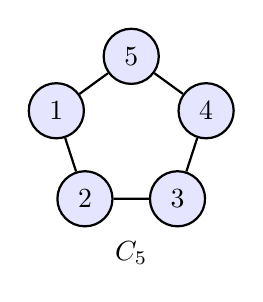
\begin{tikzpicture}[
  vnode/.style={circle, draw, minimum size=7mm, inner sep=0pt, fill=blue!10},
  thick
]
  \foreach \i in {1,2,3,4,5} {
    \node[vnode] (c\i) at ({90 + \i*360/5}:1.0) {\i};
  }
  \draw (c1) -- (c2) -- (c3) -- (c4) -- (c5) -- (c1);
  
  \node at (0, -1.5) {$C_5$};
\end{tikzpicture}
\caption{Kružnice $C_5$ s pěti vrcholy.}
\end{figure}